\chapter{Software Development}
\label{chap:software-development}

\section{Software Development Methodology}
\label{section:software-development-methodology}
<TIP: Describe your software development methodology in this section. />

\section{Technology Stack}
\label{section:technology-stack}
<TIP: Describe your technology stack here. See the following example from ThaiProgrammer.org />
\begin{figure}[h]
    \centering
    \includegraphics[width=0.5\textwidth]{examples/tech-stack.png}
    \caption{Example technology stack}
\end{figure}

\section{Coding Standards}
\label{section:coding-standards}
<TIP: Describe your coding standard for this project here. />

\section{Schedule}
\label{section:schedule}

The Prometheus project is structured into a 16-week development lifecycle. The schedule is divided into five distinct operational sections that progress from foundational infrastructure to final system evaluation, ensuring that the Computer Vision (CV) pipeline is validated before full integration with the user interfaces.

The timeline prioritizes the development of the core AI models and the Edge-to-Cloud metadata pipeline during the first half of the project. This is followed by parallel development of the iOS mobile application for members and the analytical Web Dashboard for facility owners. The final weeks are dedicated to rigorous system-wide evaluation to verify that the CV accuracy meets the established success criteria.

\begin{figure}[!ht] % [!ht] is a strong request to place it "Here" or at the "Top"
    \centering
    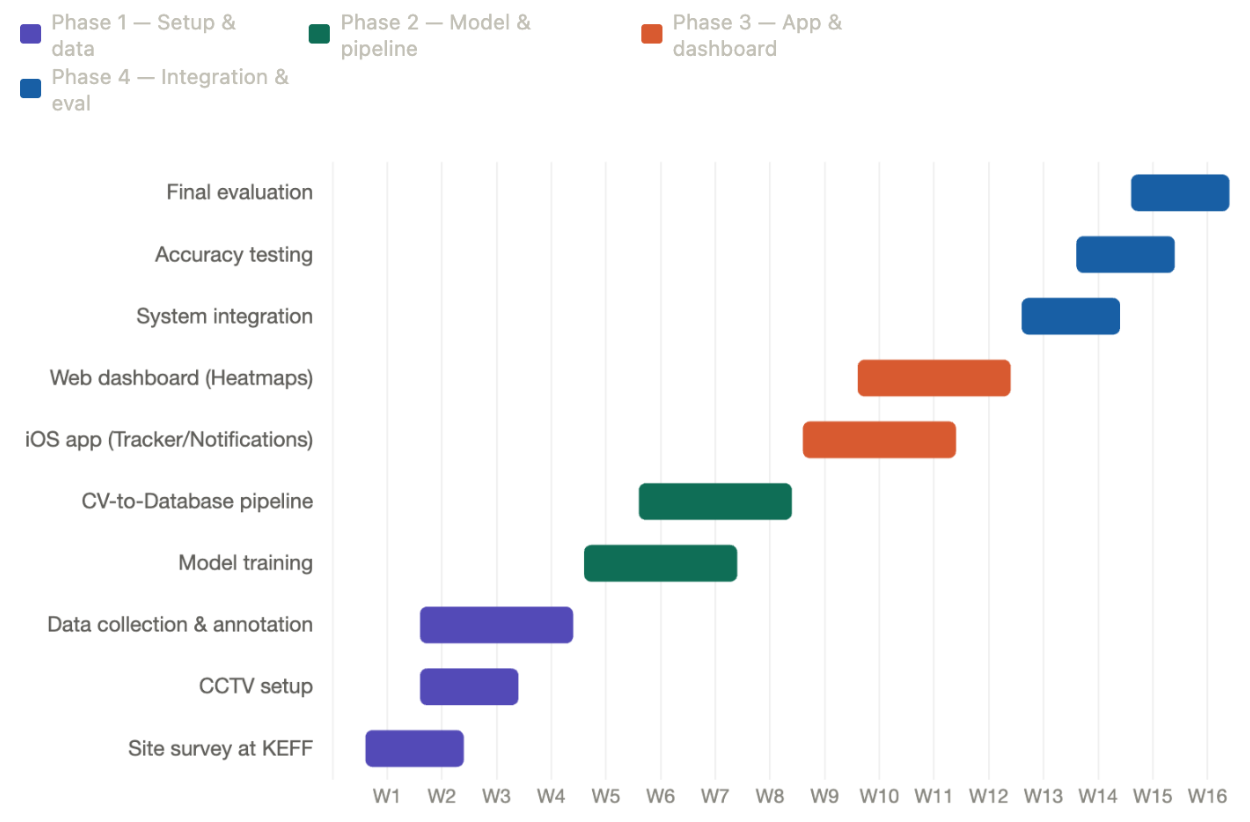
\includegraphics[width=0.9\textwidth]{assets/figures/Schedule.png}
    \caption{Prometheus Project Gantt Chart: 16-Week Development Timeline}
    \label{fig:project-schedule}
\end{figure}
\clearpage % This forces the figure to render HERE before the text below begins.

\subsection{Phase Descriptions}
Based on the visual timeline presented in the Gantt chart, the project phases are defined as follows:

\begin{itemize}
    \item \textbf{Weeks 1-4: Infrastructure Setup and Data Acquisition:} Focuses on the physical installation of the 5 HD IP cameras and the primary data collection effort necessary for training and fine-tuning the models for the specific facility layout.
    \item \textbf{Weeks 5-9: AI and Backend Core Development:} Involves the iterative training of the YOLOv10 model for machine occupancy detection and the establishment of the Edge-to-Cloud pipeline to handle anonymous metadata transmission.
    \item \textbf{Weeks 9-13: Mobile (iOS) Feature Development:} Focuses on developing the member-facing application, including the Machine Availability Tracker, the Progress Logger combined with the Diet Estimator, and the intelligent Workout Routine Generator.
    \item \textbf{Weeks 11-14: Web Dashboard Development:} Involves building the interface for gym owners, specifically the spatial heatmapping visualizations, historical utilization reports, and operational ROI tools.
    \item \textbf{Weeks 14-16: Quality Assurance and Final Evaluation:} The final phase is dedicated to validating the end-to-end system, measuring CV detection accuracy against real-world scenarios, finalizing documentation, and formal submission.
\end{itemize}

\section{Progress Tracking Report}
\label{section:progress-tracking-report}
<TIP: Show that you have been working on this project overtime.
It can be in the form of a burndown chart or a contribution graph from GitHub./>